%% fig_moduli.tex   (generated by make_diagrams.py; do not edit by hand)
%% The Weil family inside the moduli of principally polarised abelian 2n-folds: n^2 against n(2n+1), for n up to six.
\documentclass[tikz,border=8pt]{standalone}
\usepackage{amsmath,amssymb}
\usetikzlibrary{arrows.meta,calc}
%% palette.tex -- shared colour definitions for the figures
\definecolor{PInk}{RGB}{26,32,44}
\definecolor{PBlue}{RGB}{37,82,139}
\definecolor{PTeal}{RGB}{23,127,125}
\definecolor{POchre}{RGB}{193,138,44}
\definecolor{PClay}{RGB}{178,74,58}
\definecolor{PSlate}{RGB}{108,122,137}
\definecolor{PViolet}{RGB}{110,86,150}
\definecolor{WBlue}{RGB}{223,234,246}
\definecolor{WTeal}{RGB}{220,238,236}
\definecolor{WOchre}{RGB}{250,240,218}
\definecolor{WClay}{RGB}{247,229,224}
\definecolor{WSlate}{RGB}{238,241,244}
\definecolor{PMag}{RGB}{158,58,110}
\definecolor{PGrass}{RGB}{62,124,66}
\definecolor{PAmber}{RGB}{214,112,38}
\definecolor{PIndigo}{RGB}{58,64,140}
\definecolor{PRule}{RGB}{176,186,197}

%% shared macros so the standalone figures match the paper
\providecommand{\QQ}{\mathbb{Q}}
\providecommand{\ZZ}{\mathbb{Z}}
\providecommand{\RR}{\mathbb{R}}
\providecommand{\CC}{\mathbb{C}}
\providecommand{\PP}{\mathbb{P}}
\providecommand{\Kx}{K^{\times}}
\providecommand{\HW}{W}
\providecommand{\Nm}{\mathrm{N}}
\providecommand{\Hdg}{\mathrm{Hdg}}
\providecommand{\NS}{\mathrm{NS}}
\providecommand{\cA}{\mathcal{A}}
\providecommand{\cD}{\mathcal{D}}
\providecommand{\cF}{\mathcal{F}}
\providecommand{\cP}{\mathcal{P}}
\providecommand{\cO}{\mathcal{O}}
\providecommand{\cQ}{\mathcal{Q}}
\providecommand{\bbar}[1]{\overline{#1}}
\providecommand{\ch}{\operatorname{ch}}
\providecommand{\End}{\mathrm{End}}

\begin{document}
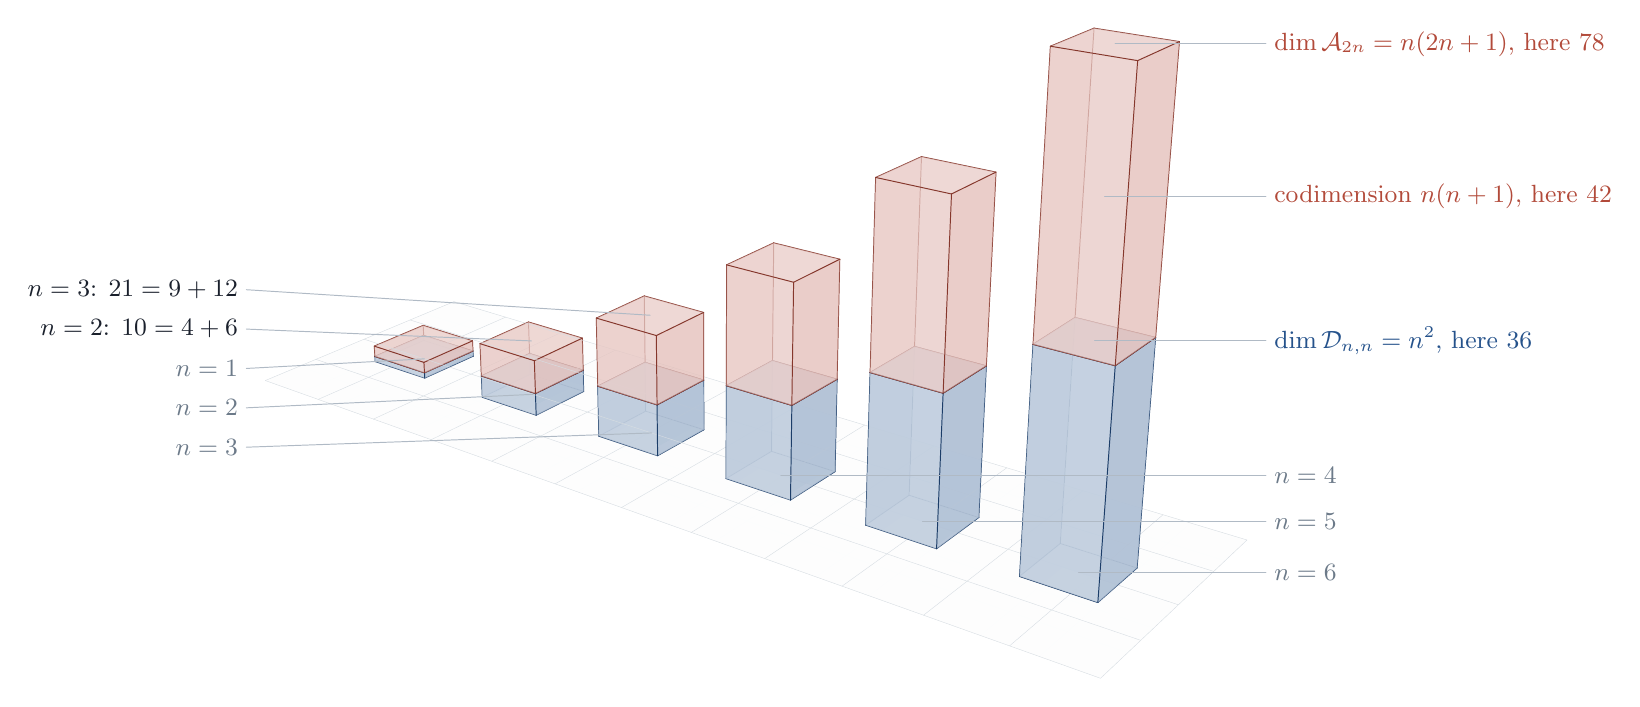
\begin{tikzpicture}[x=1cm,y=1cm,line join=round,line cap=round,
  font=\small,text=PInk]
  \path[draw=none,fill opacity=0.10,fill=PSlate!16!white] (-3.6803,-0.7652) -- (-3.2435,-0.9000) -- (-2.8770,-0.7417) -- (-3.3119,-0.6110) -- cycle;
  \path[draw=none,fill opacity=0.10,fill=PSlate!16!white] (-3.2435,-0.9000) -- (-2.7949,-1.0384) -- (-2.4305,-0.8759) -- (-2.8770,-0.7417) -- cycle;
  \path[draw=none,fill opacity=0.10,fill=PSlate!16!white] (-4.0604,-0.9241) -- (-3.6217,-1.0633) -- (-3.2435,-0.9000) -- (-3.6803,-0.7652) -- cycle;
  \path[draw=none,fill opacity=0.10,fill=PSlate!16!white] (-2.7949,-1.0384) -- (-2.3340,-1.1807) -- (-1.9720,-1.0137) -- (-2.4305,-0.8759) -- cycle;
  \path[draw=none,fill opacity=0.10,fill=PSlate!16!white] (-3.6217,-1.0633) -- (-3.1710,-1.2062) -- (-2.7949,-1.0384) -- (-3.2435,-0.9000) -- cycle;
  \path[draw=none,fill opacity=0.10,fill=PSlate!16!white] (-4.4525,-1.0882) -- (-4.0121,-1.2318) -- (-3.6217,-1.0633) -- (-4.0604,-0.9241) -- cycle;
  \draw[PRule!50,line width=0.15pt] (-5.7077,-1.6133) -- (-3.3119,-0.6110);
  \draw[PBlue!75!black,line width=0.35pt] (-3.6921,-1.1045) -- (-3.6955,-1.0407);
  \draw[PClay!75!black,line width=0.35pt] (-3.6955,-1.0407) -- (-3.7023,-0.9129);
  \path[draw=none,fill opacity=0.10,fill=PSlate!16!white] (-2.3340,-1.1807) -- (-1.8604,-1.3268) -- (-1.5010,-1.1553) -- (-1.9720,-1.0137) -- cycle;
  \path[draw=none,fill opacity=0.10,fill=PSlate!16!white] (-3.1710,-1.2062) -- (-2.7079,-1.3531) -- (-2.3340,-1.1807) -- (-2.7949,-1.0384) -- cycle;
  \draw[PBlue!75!black,line width=0.35pt] (-3.6921,-1.1045) -- (-3.0674,-1.3038);
  \path[draw=none,fill opacity=0.78,fill=PBlue!28!white] (-3.6921,-1.1045) -- (-3.0674,-1.3038) -- (-3.0703,-1.2390) -- (-3.6955,-1.0407) -- cycle;
  \draw[PBlue!75!black,line width=0.35pt] (-3.6955,-1.0407) -- (-3.0703,-1.2390);
  \draw[PClay!75!black,line width=0.35pt] (-3.6955,-1.0407) -- (-3.0703,-1.2390);
  \path[draw=none,fill opacity=0.10,fill=PSlate!16!white] (-4.0121,-1.2318) -- (-3.5595,-1.3794) -- (-3.1710,-1.2062) -- (-3.6217,-1.0633) -- cycle;
  \path[draw=none,fill opacity=0.55,fill=PClay!28!white] (-3.6955,-1.0407) -- (-3.0703,-1.2390) -- (-3.0760,-1.1091) -- (-3.7023,-0.9129) -- cycle;
  \draw[PClay!75!black,line width=0.35pt] (-3.7023,-0.9129) -- (-3.0760,-1.1091);
  \draw[PBlue!75!black,line width=0.35pt] (-4.3111,-1.3719) -- (-3.6921,-1.1045);
  \path[draw=none,fill opacity=0.78,fill=PBlue!37!white] (-4.3111,-1.3719) -- (-3.6921,-1.1045) -- (-3.6955,-1.0407) -- (-4.3151,-1.3068) -- cycle;
  \path[draw=none,fill opacity=0.10,fill=PSlate!16!white] (-4.8573,-1.2576) -- (-4.4154,-1.4059) -- (-4.0121,-1.2318) -- (-4.4525,-1.0882) -- cycle;
  \draw[PBlue!75!black,line width=0.35pt] (-4.3151,-1.3068) -- (-3.6955,-1.0407);
  \draw[PClay!75!black,line width=0.35pt] (-4.3151,-1.3068) -- (-3.6955,-1.0407);
  \path[draw=none,fill opacity=0.55,fill=PClay!37!white] (-4.3151,-1.3068) -- (-3.6955,-1.0407) -- (-3.7023,-0.9129) -- (-4.3232,-1.1762) -- cycle;
  \draw[PClay!75!black,line width=0.35pt] (-4.3232,-1.1762) -- (-3.7023,-0.9129);
  \draw[PRule!50,line width=0.15pt] (-5.0358,-1.8528) -- (-2.6552,-0.8084);
  \draw[PBlue!75!black,line width=0.35pt] (-3.0674,-1.3038) -- (-3.0703,-1.2390);
  \path[draw=none,fill opacity=0.10,fill=PSlate!16!white] (-1.8604,-1.3268) -- (-1.3734,-1.4771) -- (-1.0170,-1.3008) -- (-1.5010,-1.1553) -- cycle;
  \draw[PClay!75!black,line width=0.35pt] (-3.0703,-1.2390) -- (-3.0760,-1.1091);
  \path[draw=none,fill opacity=0.78,fill=PBlue!26!white] (-4.3111,-1.3719) -- (-3.6822,-1.5817) -- (-3.0674,-1.3038) -- (-3.6921,-1.1045) -- cycle;
  \path[draw=none,fill opacity=0.10,fill=PSlate!16!white] (-2.7079,-1.3531) -- (-2.2316,-1.5041) -- (-1.8604,-1.3268) -- (-2.3340,-1.1807) -- cycle;
  \path[draw=none,fill opacity=0.78,fill=PBlue!26!white] (-4.3151,-1.3068) -- (-3.6857,-1.5155) -- (-3.0703,-1.2390) -- (-3.6955,-1.0407) -- cycle;
  \path[draw=none,fill opacity=0.55,fill=PClay!26!white] (-4.3151,-1.3068) -- (-3.6857,-1.5155) -- (-3.0703,-1.2390) -- (-3.6955,-1.0407) -- cycle;
  \path[draw=none,fill opacity=0.10,fill=PSlate!16!white] (-3.5595,-1.3794) -- (-3.0941,-1.5312) -- (-2.7079,-1.3531) -- (-3.1710,-1.2062) -- cycle;
  \path[draw=none,fill opacity=0.55,fill=PClay!26!white] (-4.3232,-1.1762) -- (-3.6928,-1.3827) -- (-3.0760,-1.1091) -- (-3.7023,-0.9129) -- cycle;
  \draw[PBlue!75!black,line width=0.35pt] (-4.3111,-1.3719) -- (-4.3151,-1.3068);
  \draw[PClay!75!black,line width=0.35pt] (-4.3151,-1.3068) -- (-4.3232,-1.1762);
  \path[draw=none,fill opacity=0.10,fill=PSlate!16!white] (-4.4154,-1.4059) -- (-3.9610,-1.5584) -- (-3.5595,-1.3794) -- (-4.0121,-1.2318) -- cycle;
  \path[draw=none,fill opacity=0.10,fill=PSlate!16!white] (-5.2755,-1.4325) -- (-4.8321,-1.5858) -- (-4.4154,-1.4059) -- (-4.8573,-1.2576) -- cycle;
  \draw[PBlue!75!black,line width=0.35pt] (-3.6822,-1.5817) -- (-3.0674,-1.3038);
  \path[draw=none,fill opacity=0.78,fill=PBlue!37!white] (-3.6822,-1.5817) -- (-3.0674,-1.3038) -- (-3.0703,-1.2390) -- (-3.6857,-1.5155) -- cycle;
  \draw[PBlue!75!black,line width=0.35pt] (-3.6857,-1.5155) -- (-3.0703,-1.2390);
  \draw[PClay!75!black,line width=0.35pt] (-3.6857,-1.5155) -- (-3.0703,-1.2390);
  \path[draw=none,fill opacity=0.55,fill=PClay!37!white] (-3.6857,-1.5155) -- (-3.0703,-1.2390) -- (-3.0760,-1.1091) -- (-3.6928,-1.3827) -- cycle;
  \path[draw=none,fill opacity=0.10,fill=PSlate!16!white] (-1.3734,-1.4771) -- (-0.8725,-1.6317) -- (-0.5194,-1.4503) -- (-1.0170,-1.3008) -- cycle;
  \draw[PClay!75!black,line width=0.35pt] (-3.6928,-1.3827) -- (-3.0760,-1.1091);
  \draw[PBlue!75!black,line width=0.35pt] (-4.3111,-1.3719) -- (-3.6822,-1.5817);
  \path[draw=none,fill opacity=0.78,fill=PBlue!28!white] (-4.3111,-1.3719) -- (-3.6822,-1.5817) -- (-3.6857,-1.5155) -- (-4.3151,-1.3068) -- cycle;
  \draw[PBlue!75!black,line width=0.35pt] (-4.3151,-1.3068) -- (-3.6857,-1.5155);
  \draw[PClay!75!black,line width=0.35pt] (-4.3151,-1.3068) -- (-3.6857,-1.5155);
  \path[draw=none,fill opacity=0.10,fill=PSlate!16!white] (-2.2316,-1.5041) -- (-1.7418,-1.6594) -- (-1.3734,-1.4771) -- (-1.8604,-1.3268) -- cycle;
  \path[draw=none,fill opacity=0.55,fill=PClay!28!white] (-4.3151,-1.3068) -- (-3.6857,-1.5155) -- (-3.6928,-1.3827) -- (-4.3232,-1.1762) -- cycle;
  \draw[PClay!75!black,line width=0.35pt] (-4.3232,-1.1762) -- (-3.6928,-1.3827);
  \path[draw=none,fill opacity=0.10,fill=PSlate!16!white] (-3.0941,-1.5312) -- (-2.6154,-1.6873) -- (-2.2316,-1.5041) -- (-2.7079,-1.3531) -- cycle;
  \draw[PRule!50,line width=0.15pt] (-4.3340,-2.1030) -- (-1.9720,-1.0137);
  \path[draw=none,fill opacity=0.10,fill=PSlate!16!white] (-3.9610,-1.5584) -- (-3.4935,-1.7153) -- (-3.0941,-1.5312) -- (-3.5595,-1.3794) -- cycle;
  \draw[PBlue!75!black,line width=0.35pt] (-2.3420,-1.5353) -- (-2.3509,-1.2706);
  \path[draw=none,fill opacity=0.10,fill=PSlate!16!white] (-4.8321,-1.5858) -- (-4.3760,-1.7435) -- (-3.9610,-1.5584) -- (-4.4154,-1.4059) -- cycle;
  \draw[PBlue!75!black,line width=0.35pt] (-3.6822,-1.5817) -- (-3.6857,-1.5155);
  \path[draw=none,fill opacity=0.10,fill=PSlate!16!white] (-5.7077,-1.6133) -- (-5.2630,-1.7718) -- (-4.8321,-1.5858) -- (-5.2755,-1.4325) -- cycle;
  \draw[PClay!75!black,line width=0.35pt] (-3.6857,-1.5155) -- (-3.6928,-1.3827);
  \draw[PClay!75!black,line width=0.35pt] (-2.3509,-1.2706) -- (-2.3645,-0.8699);
  \path[draw=none,fill opacity=0.10,fill=PSlate!16!white] (-0.8725,-1.6317) -- (-0.3572,-1.7907) -- (-0.0076,-1.6041) -- (-0.5194,-1.4503) -- cycle;
  \draw[PBlue!75!black,line width=0.35pt] (-2.3420,-1.5353) -- (-1.6642,-1.7515);
  \path[draw=none,fill opacity=0.10,fill=PSlate!16!white] (-1.7418,-1.6594) -- (-1.2377,-1.8193) -- (-0.8725,-1.6317) -- (-1.3734,-1.4771) -- cycle;
  \path[draw=none,fill opacity=0.78,fill=PBlue!28!white] (-2.3420,-1.5353) -- (-1.6642,-1.7515) -- (-1.6707,-1.4824) -- (-2.3509,-1.2706) -- cycle;
  \path[draw=none,fill opacity=0.10,fill=PSlate!16!white] (-2.6154,-1.6873) -- (-2.1227,-1.8480) -- (-1.7418,-1.6594) -- (-2.2316,-1.5041) -- cycle;
  \draw[PBlue!75!black,line width=0.35pt] (-2.9511,-1.8255) -- (-2.3420,-1.5353);
  \draw[PBlue!75!black,line width=0.35pt] (-2.3509,-1.2706) -- (-1.6707,-1.4824);
  \draw[PClay!75!black,line width=0.35pt] (-2.3509,-1.2706) -- (-1.6707,-1.4824);
  \path[draw=none,fill opacity=0.78,fill=PBlue!37!white] (-2.9511,-1.8255) -- (-2.3420,-1.5353) -- (-2.3509,-1.2706) -- (-2.9627,-1.5549) -- cycle;
  \path[draw=none,fill opacity=0.10,fill=PSlate!16!white] (-3.4935,-1.7153) -- (-3.0123,-1.8768) -- (-2.6154,-1.6873) -- (-3.0941,-1.5312) -- cycle;
  \path[draw=none,fill opacity=0.55,fill=PClay!28!white] (-2.3509,-1.2706) -- (-1.6707,-1.4824) -- (-1.6806,-1.0749) -- (-2.3645,-0.8699) -- cycle;
  \draw[PBlue!75!black,line width=0.35pt] (-2.9627,-1.5549) -- (-2.3509,-1.2706);
  \draw[PClay!75!black,line width=0.35pt] (-2.9627,-1.5549) -- (-2.3509,-1.2706);
  \path[draw=none,fill opacity=0.10,fill=PSlate!16!white] (-4.3760,-1.7435) -- (-3.9065,-1.9058) -- (-3.4935,-1.7153) -- (-3.9610,-1.5584) -- cycle;
  \draw[PClay!75!black,line width=0.35pt] (-2.3645,-0.8699) -- (-1.6806,-1.0749);
  \path[draw=none,fill opacity=0.55,fill=PClay!37!white] (-2.9627,-1.5549) -- (-2.3509,-1.2706) -- (-2.3645,-0.8699) -- (-2.9802,-1.1451) -- cycle;
  \path[draw=none,fill opacity=0.10,fill=PSlate!16!white] (-5.2630,-1.7718) -- (-4.8053,-1.9350) -- (-4.3760,-1.7435) -- (-4.8321,-1.5858) -- cycle;
  \draw[PRule!50,line width=0.15pt] (-3.6002,-2.3645) -- (-1.2607,-1.2275);
  \draw[PBlue!75!black,line width=0.35pt] (-1.6642,-1.7515) -- (-1.6707,-1.4824);
  \path[draw=none,fill opacity=0.10,fill=PSlate!16!white] (-0.3572,-1.7907) -- (0.1733,-1.9545) -- (0.5189,-1.7623) -- (-0.0076,-1.6041) -- cycle;
  \draw[PClay!75!black,line width=0.35pt] (-2.9802,-1.1451) -- (-2.3645,-0.8699);
  \path[draw=none,fill opacity=0.78,fill=PBlue!26!white] (-2.9511,-1.8255) -- (-2.2673,-2.0535) -- (-1.6642,-1.7515) -- (-2.3420,-1.5353) -- cycle;
  \path[draw=none,fill opacity=0.10,fill=PSlate!16!white] (-1.2377,-1.8193) -- (-0.7188,-1.9839) -- (-0.3572,-1.7907) -- (-0.8725,-1.6317) -- cycle;
  \draw[PClay!75!black,line width=0.35pt] (-1.6707,-1.4824) -- (-1.6806,-1.0749);
  \path[draw=none,fill opacity=0.78,fill=PBlue!26!white] (-2.9627,-1.5549) -- (-2.2764,-1.7783) -- (-1.6707,-1.4824) -- (-2.3509,-1.2706) -- cycle;
  \path[draw=none,fill opacity=0.55,fill=PClay!26!white] (-2.9627,-1.5549) -- (-2.2764,-1.7783) -- (-1.6707,-1.4824) -- (-2.3509,-1.2706) -- cycle;
  \path[draw=none,fill opacity=0.10,fill=PSlate!16!white] (-2.1227,-1.8480) -- (-1.6155,-2.0134) -- (-1.2377,-1.8193) -- (-1.7418,-1.6594) -- cycle;
  \draw[PBlue!75!black,line width=0.35pt] (-2.9511,-1.8255) -- (-2.9627,-1.5549);
  \path[draw=none,fill opacity=0.10,fill=PSlate!16!white] (-3.0123,-1.8768) -- (-2.5170,-2.0431) -- (-2.1227,-1.8480) -- (-2.6154,-1.6873) -- cycle;
  \path[draw=none,fill opacity=0.10,fill=PSlate!16!white] (-3.9065,-1.9058) -- (-3.4231,-2.0729) -- (-3.0123,-1.8768) -- (-3.4935,-1.7153) -- cycle;
  \path[draw=none,fill opacity=0.55,fill=PClay!26!white] (-2.9802,-1.1451) -- (-2.2902,-1.3614) -- (-1.6806,-1.0749) -- (-2.3645,-0.8699) -- cycle;
  \draw[PBlue!75!black,line width=0.35pt] (-2.2673,-2.0535) -- (-1.6642,-1.7515);
  \draw[PClay!75!black,line width=0.35pt] (-2.9627,-1.5549) -- (-2.9802,-1.1451);
  \path[draw=none,fill opacity=0.10,fill=PSlate!16!white] (-4.8053,-1.9350) -- (-4.3340,-2.1030) -- (-3.9065,-1.9058) -- (-4.3760,-1.7435) -- cycle;
  \path[draw=none,fill opacity=0.78,fill=PBlue!37!white] (-2.2673,-2.0535) -- (-1.6642,-1.7515) -- (-1.6707,-1.4824) -- (-2.2764,-1.7783) -- cycle;
  \draw[PRule!50,line width=0.15pt] (-3.3119,-0.6110) -- (6.7606,-3.6382);
  \draw[PBlue!75!black,line width=0.35pt] (-2.9511,-1.8255) -- (-2.2673,-2.0535);
  \path[draw=none,fill opacity=0.10,fill=PSlate!16!white] (0.1733,-1.9545) -- (0.7196,-2.1231) -- (1.0608,-1.9252) -- (0.5189,-1.7623) -- cycle;
  \draw[PBlue!75!black,line width=0.35pt] (-2.2764,-1.7783) -- (-1.6707,-1.4824);
  \draw[PClay!75!black,line width=0.35pt] (-2.2764,-1.7783) -- (-1.6707,-1.4824);
  \path[draw=none,fill opacity=0.78,fill=PBlue!28!white] (-2.9511,-1.8255) -- (-2.2673,-2.0535) -- (-2.2764,-1.7783) -- (-2.9627,-1.5549) -- cycle;
  \path[draw=none,fill opacity=0.10,fill=PSlate!16!white] (-0.7188,-1.9839) -- (-0.1844,-2.1533) -- (0.1733,-1.9545) -- (-0.3572,-1.7907) -- cycle;
  \path[draw=none,fill opacity=0.55,fill=PClay!37!white] (-2.2764,-1.7783) -- (-1.6707,-1.4824) -- (-1.6806,-1.0749) -- (-2.2902,-1.3614) -- cycle;
  \draw[PBlue!75!black,line width=0.35pt] (-2.9627,-1.5549) -- (-2.2764,-1.7783);
  \draw[PClay!75!black,line width=0.35pt] (-2.9627,-1.5549) -- (-2.2764,-1.7783);
  \path[draw=none,fill opacity=0.10,fill=PSlate!16!white] (-1.6155,-2.0134) -- (-1.0932,-2.1838) -- (-0.7188,-1.9839) -- (-1.2377,-1.8193) -- cycle;
  \draw[PClay!75!black,line width=0.35pt] (-2.2902,-1.3614) -- (-1.6806,-1.0749);
  \draw[PRule!50,line width=0.15pt] (-2.8321,-2.6383) -- (-0.5194,-1.4503);
  \path[draw=none,fill opacity=0.55,fill=PClay!28!white] (-2.9627,-1.5549) -- (-2.2764,-1.7783) -- (-2.2902,-1.3614) -- (-2.9802,-1.1451) -- cycle;
  \path[draw=none,fill opacity=0.10,fill=PSlate!16!white] (-2.5170,-2.0431) -- (-2.0067,-2.2144) -- (-1.6155,-2.0134) -- (-2.1227,-1.8480) -- cycle;
  \draw[PClay!75!black,line width=0.35pt] (-2.9802,-1.1451) -- (-2.2902,-1.3614);
  \draw[PBlue!75!black,line width=0.35pt] (-0.8759,-2.0030) -- (-0.8838,-1.3831);
  \path[draw=none,fill opacity=0.10,fill=PSlate!16!white] (-3.4231,-2.0729) -- (-2.9252,-2.2451) -- (-2.5170,-2.0431) -- (-3.0123,-1.8768) -- cycle;
  \draw[PBlue!75!black,line width=0.35pt] (-2.2673,-2.0535) -- (-2.2764,-1.7783);
  \path[draw=none,fill opacity=0.10,fill=PSlate!16!white] (-4.3340,-2.1030) -- (-3.8485,-2.2760) -- (-3.4231,-2.0729) -- (-3.9065,-1.9058) -- cycle;
  \path[draw=none,fill opacity=0.10,fill=PSlate!16!white] (0.7196,-2.1231) -- (1.2824,-2.2967) -- (1.6189,-2.0929) -- (1.0608,-1.9252) -- cycle;
  \draw[PBlue!75!black,line width=0.35pt] (-0.8759,-2.0030) -- (-0.1381,-2.2384);
  \draw[PClay!75!black,line width=0.35pt] (-2.2764,-1.7783) -- (-2.2902,-1.3614);
  \path[draw=none,fill opacity=0.10,fill=PSlate!16!white] (-0.1844,-2.1533) -- (0.3662,-2.3279) -- (0.7196,-2.1231) -- (0.1733,-1.9545) -- cycle;
  \draw[PBlue!75!black,line width=0.35pt] (-1.4711,-2.3191) -- (-0.8759,-2.0030);
  \path[draw=none,fill opacity=0.10,fill=PSlate!16!white] (-1.0932,-2.1838) -- (-0.5549,-2.3593) -- (-0.1844,-2.1533) -- (-0.7188,-1.9839) -- cycle;
  \path[draw=none,fill opacity=0.78,fill=PBlue!28!white] (-0.8759,-2.0030) -- (-0.1381,-2.2384) -- (-0.1394,-1.6077) -- (-0.8838,-1.3831) -- cycle;
  \draw[PClay!75!black,line width=0.35pt] (-0.8838,-1.3831) -- (-0.8945,-0.5388);
  \path[draw=none,fill opacity=0.10,fill=PSlate!16!white] (-2.0067,-2.2144) -- (-1.4809,-2.3908) -- (-1.0932,-2.1838) -- (-1.6155,-2.0134) -- cycle;
  \path[draw=none,fill opacity=0.78,fill=PBlue!37!white] (-1.4711,-2.3191) -- (-0.8759,-2.0030) -- (-0.8838,-1.3831) -- (-1.4847,-1.6847) -- cycle;
  \draw[PBlue!75!black,line width=0.35pt] (-0.8838,-1.3831) -- (-0.1394,-1.6077);
  \draw[PClay!75!black,line width=0.35pt] (-0.8838,-1.3831) -- (-0.1394,-1.6077);
  \draw[PRule!50,line width=0.15pt] (-3.8689,-0.8440) -- (6.3383,-4.0370);
  \path[draw=none,fill opacity=0.10,fill=PSlate!16!white] (-2.9252,-2.2451) -- (-2.4120,-2.4225) -- (-2.0067,-2.2144) -- (-2.5170,-2.0431) -- cycle;
  \path[draw=none,fill opacity=0.10,fill=PSlate!16!white] (-3.8485,-2.2760) -- (-3.3481,-2.4544) -- (-2.9252,-2.2451) -- (-3.4231,-2.0729) -- cycle;
  \draw[PBlue!75!black,line width=0.35pt] (-1.4847,-1.6847) -- (-0.8838,-1.3831);
  \draw[PClay!75!black,line width=0.35pt] (-1.4847,-1.6847) -- (-0.8838,-1.3831);
  \draw[PRule!50,line width=0.15pt] (-2.0273,-2.9252) -- (0.2537,-1.6827);
  \path[draw=none,fill opacity=0.78,fill=PBlue!26!white] (-1.4711,-2.3191) -- (-0.7250,-2.5679) -- (-0.1381,-2.2384) -- (-0.8759,-2.0030) -- cycle;
  \path[draw=none,fill opacity=0.10,fill=PSlate!16!white] (1.2824,-2.2967) -- (1.8625,-2.4758) -- (2.1937,-2.2657) -- (1.6189,-2.0929) -- cycle;
  \draw[PBlue!75!black,line width=0.35pt] (-0.1381,-2.2384) -- (-0.1394,-1.6077);
  \path[draw=none,fill opacity=0.55,fill=PClay!28!white] (-0.8838,-1.3831) -- (-0.1394,-1.6077) -- (-0.1411,-0.7484) -- (-0.8945,-0.5388) -- cycle;
  \path[draw=none,fill opacity=0.10,fill=PSlate!16!white] (0.3662,-2.3279) -- (0.9338,-2.5079) -- (1.2824,-2.2967) -- (0.7196,-2.1231) -- cycle;
  \path[draw=none,fill opacity=0.55,fill=PClay!37!white] (-1.4847,-1.6847) -- (-0.8838,-1.3831) -- (-0.8945,-0.5388) -- (-1.5034,-0.8202) -- cycle;
  \path[draw=none,fill opacity=0.10,fill=PSlate!16!white] (-0.5549,-2.3593) -- (0.0000,-2.5403) -- (0.3662,-2.3279) -- (-0.1844,-2.1533) -- cycle;
  \draw[PClay!75!black,line width=0.35pt] (-0.8945,-0.5388) -- (-0.1411,-0.7484);
  \draw[PBlue!75!black,line width=0.35pt] (-1.4711,-2.3191) -- (-1.4847,-1.6847);
  \path[draw=none,fill opacity=0.10,fill=PSlate!16!white] (-1.4809,-2.3908) -- (-0.9389,-2.5728) -- (-0.5549,-2.3593) -- (-1.0932,-2.1838) -- cycle;
  \path[draw=none,fill opacity=0.78,fill=PBlue!26!white] (-1.4847,-1.6847) -- (-0.7319,-1.9222) -- (-0.1394,-1.6077) -- (-0.8838,-1.3831) -- cycle;
  \path[draw=none,fill opacity=0.55,fill=PClay!26!white] (-1.4847,-1.6847) -- (-0.7319,-1.9222) -- (-0.1394,-1.6077) -- (-0.8838,-1.3831) -- cycle;
  \draw[PBlue!75!black,line width=0.35pt] (-0.7250,-2.5679) -- (-0.1381,-2.2384);
  \path[draw=none,fill opacity=0.10,fill=PSlate!16!white] (-2.4120,-2.4225) -- (-1.8829,-2.6055) -- (-1.4809,-2.3908) -- (-2.0067,-2.2144) -- cycle;
  \draw[PClay!75!black,line width=0.35pt] (-1.5034,-0.8202) -- (-0.8945,-0.5388);
  \draw[PClay!75!black,line width=0.35pt] (-0.1394,-1.6077) -- (-0.1411,-0.7484);
  \path[draw=none,fill opacity=0.10,fill=PSlate!16!white] (-3.3481,-2.4544) -- (-2.8321,-2.6383) -- (-2.4120,-2.4225) -- (-2.9252,-2.2451) -- cycle;
  \draw[PBlue!75!black,line width=0.35pt] (-1.4711,-2.3191) -- (-0.7250,-2.5679);
  \path[draw=none,fill opacity=0.78,fill=PBlue!37!white] (-0.7250,-2.5679) -- (-0.1381,-2.2384) -- (-0.1394,-1.6077) -- (-0.7319,-1.9222) -- cycle;
  \path[draw=none,fill opacity=0.10,fill=PSlate!16!white] (1.8625,-2.4758) -- (2.4607,-2.6604) -- (2.7862,-2.4438) -- (2.1937,-2.2657) -- cycle;
  \path[draw=none,fill opacity=0.10,fill=PSlate!16!white] (0.9338,-2.5079) -- (1.5191,-2.6935) -- (1.8625,-2.4758) -- (1.2824,-2.2967) -- cycle;
  \path[draw=none,fill opacity=0.78,fill=PBlue!28!white] (-1.4711,-2.3191) -- (-0.7250,-2.5679) -- (-0.7319,-1.9222) -- (-1.4847,-1.6847) -- cycle;
  \draw[PClay!75!black,line width=0.35pt] (-1.4847,-1.6847) -- (-1.5034,-0.8202);
  \draw[PBlue!75!black,line width=0.35pt] (-0.7319,-1.9222) -- (-0.1394,-1.6077);
  \draw[PClay!75!black,line width=0.35pt] (-0.7319,-1.9222) -- (-0.1394,-1.6077);
  \path[draw=none,fill opacity=0.10,fill=PSlate!16!white] (0.0000,-2.5403) -- (0.5723,-2.7269) -- (0.9338,-2.5079) -- (0.3662,-2.3279) -- cycle;
  \path[draw=none,fill opacity=0.55,fill=PClay!26!white] (-1.5034,-0.8202) -- (-0.7413,-1.0420) -- (-0.1411,-0.7484) -- (-0.8945,-0.5388) -- cycle;
  \draw[PRule!50,line width=0.15pt] (-1.1831,-3.2262) -- (1.0608,-1.9252);
  \draw[PRule!50,line width=0.15pt] (-4.4525,-1.0882) -- (5.8892,-4.4609);
  \draw[PBlue!75!black,line width=0.35pt] (-1.4847,-1.6847) -- (-0.7319,-1.9222);
  \draw[PClay!75!black,line width=0.35pt] (-1.4847,-1.6847) -- (-0.7319,-1.9222);
  \path[draw=none,fill opacity=0.10,fill=PSlate!16!white] (-0.9389,-2.5728) -- (-0.3798,-2.7604) -- (0.0000,-2.5403) -- (-0.5549,-2.3593) -- cycle;
  \path[draw=none,fill opacity=0.55,fill=PClay!37!white] (-0.7319,-1.9222) -- (-0.1394,-1.6077) -- (-0.1411,-0.7484) -- (-0.7413,-1.0420) -- cycle;
  \path[draw=none,fill opacity=0.10,fill=PSlate!16!white] (-1.8829,-2.6055) -- (-1.3371,-2.7942) -- (-0.9389,-2.5728) -- (-1.4809,-2.3908) -- cycle;
  \draw[PBlue!75!black,line width=0.35pt] (0.7217,-2.5128) -- (0.7339,-1.3608);
  \path[draw=none,fill opacity=0.10,fill=PSlate!16!white] (-2.8321,-2.6383) -- (-2.2998,-2.8281) -- (-1.8829,-2.6055) -- (-2.4120,-2.4225) -- cycle;
  \draw[PBlue!75!black,line width=0.35pt] (-0.7250,-2.5679) -- (-0.7319,-1.9222);
  \path[draw=none,fill opacity=0.55,fill=PClay!28!white] (-1.4847,-1.6847) -- (-0.7319,-1.9222) -- (-0.7413,-1.0420) -- (-1.5034,-0.8202) -- cycle;
  \draw[PBlue!75!black,line width=0.35pt] (0.7217,-2.5128) -- (1.5279,-2.7700);
  \path[draw=none,fill opacity=0.10,fill=PSlate!16!white] (2.4607,-2.6604) -- (3.0778,-2.8508) -- (3.3971,-2.6274) -- (2.7862,-2.4438) -- cycle;
  \draw[PClay!75!black,line width=0.35pt] (-0.7413,-1.0420) -- (-0.1411,-0.7484);
  \path[draw=none,fill opacity=0.10,fill=PSlate!16!white] (1.5191,-2.6935) -- (2.1230,-2.8851) -- (2.4607,-2.6604) -- (1.8625,-2.4758) -- cycle;
  \draw[PBlue!75!black,line width=0.35pt] (0.1455,-2.8582) -- (0.7217,-2.5128);
  \draw[PClay!75!black,line width=0.35pt] (-1.5034,-0.8202) -- (-0.7413,-1.0420);
  \path[draw=none,fill opacity=0.10,fill=PSlate!16!white] (0.5723,-2.7269) -- (1.1628,-2.9195) -- (1.5191,-2.6935) -- (0.9338,-2.5079) -- cycle;
  \path[draw=none,fill opacity=0.78,fill=PBlue!28!white] (0.7217,-2.5128) -- (1.5279,-2.7700) -- (1.5543,-1.5971) -- (0.7339,-1.3608) -- cycle;
  \path[draw=none,fill opacity=0.10,fill=PSlate!16!white] (-0.3798,-2.7604) -- (0.1972,-2.9541) -- (0.5723,-2.7269) -- (0.0000,-2.5403) -- cycle;
  \draw[PClay!75!black,line width=0.35pt] (-0.7319,-1.9222) -- (-0.7413,-1.0420);
  \path[draw=none,fill opacity=0.10,fill=PSlate!16!white] (-1.3371,-2.7942) -- (-0.7739,-2.9889) -- (-0.3798,-2.7604) -- (-0.9389,-2.5728) -- cycle;
  \path[draw=none,fill opacity=0.78,fill=PBlue!37!white] (0.1455,-2.8582) -- (0.7217,-2.5128) -- (0.7339,-1.3608) -- (0.1480,-1.6782) -- cycle;
  \path[draw=none,fill opacity=0.10,fill=PSlate!16!white] (-2.2998,-2.8281) -- (-1.7504,-3.0239) -- (-1.3371,-2.7942) -- (-1.8829,-2.6055) -- cycle;
  \path[draw=none,fill opacity=0.78,fill=PBlue!26!white] (0.1455,-2.8582) -- (0.9628,-3.1308) -- (1.5279,-2.7700) -- (0.7217,-2.5128) -- cycle;
  \draw[PRule!50,line width=0.15pt] (-0.2965,-3.5422) -- (1.9041,-2.1787);
  \path[draw=none,fill opacity=0.10,fill=PSlate!16!white] (3.0778,-2.8508) -- (3.7148,-3.0474) -- (4.0273,-2.8168) -- (3.3971,-2.6274) -- cycle;
  \draw[PClay!75!black,line width=0.35pt] (0.7339,-1.3608) -- (0.7497,0.1350);
  \draw[PBlue!75!black,line width=0.35pt] (0.7339,-1.3608) -- (1.5543,-1.5971);
  \draw[PClay!75!black,line width=0.35pt] (0.7339,-1.3608) -- (1.5543,-1.5971);
  \path[draw=none,fill opacity=0.10,fill=PSlate!16!white] (2.1230,-2.8851) -- (2.7464,-3.0828) -- (3.0778,-2.8508) -- (2.4607,-2.6604) -- cycle;
  \draw[PRule!50,line width=0.15pt] (-5.0647,-1.3443) -- (5.4109,-4.9125);
  \draw[PBlue!75!black,line width=0.35pt] (1.5279,-2.7700) -- (1.5543,-1.5971);
  \draw[PBlue!75!black,line width=0.35pt] (0.1480,-1.6782) -- (0.7339,-1.3608);
  \draw[PClay!75!black,line width=0.35pt] (0.1480,-1.6782) -- (0.7339,-1.3608);
  \path[draw=none,fill opacity=0.10,fill=PSlate!16!white] (1.1628,-2.9195) -- (1.7724,-3.1183) -- (2.1230,-2.8851) -- (1.5191,-2.6935) -- cycle;
  \path[draw=none,fill opacity=0.10,fill=PSlate!16!white] (0.1972,-2.9541) -- (0.7929,-3.1541) -- (1.1628,-2.9195) -- (0.5723,-2.7269) -- cycle;
  \draw[PBlue!75!black,line width=0.35pt] (0.9628,-3.1308) -- (1.5279,-2.7700);
  \draw[PBlue!75!black,line width=0.35pt] (0.1455,-2.8582) -- (0.1480,-1.6782);
  \path[draw=none,fill opacity=0.10,fill=PSlate!16!white] (-0.7739,-2.9889) -- (-0.1922,-3.1900) -- (0.1972,-2.9541) -- (-0.3798,-2.7604) -- cycle;
  \path[draw=none,fill opacity=0.55,fill=PClay!28!white] (0.7339,-1.3608) -- (1.5543,-1.5971) -- (1.5886,-0.0728) -- (0.7497,0.1350) -- cycle;
  \draw[PBlue!75!black,line width=0.35pt] (0.1455,-2.8582) -- (0.9628,-3.1308);
  \path[draw=none,fill opacity=0.10,fill=PSlate!16!white] (-1.7504,-3.0239) -- (-1.1831,-3.2262) -- (-0.7739,-2.9889) -- (-1.3371,-2.7942) -- cycle;
  \path[draw=none,fill opacity=0.55,fill=PClay!37!white] (0.1480,-1.6782) -- (0.7339,-1.3608) -- (0.7497,0.1350) -- (0.1513,-0.1441) -- cycle;
  \path[draw=none,fill opacity=0.78,fill=PBlue!26!white] (0.1480,-1.6782) -- (0.9799,-1.9288) -- (1.5543,-1.5971) -- (0.7339,-1.3608) -- cycle;
  \path[draw=none,fill opacity=0.55,fill=PClay!26!white] (0.1480,-1.6782) -- (0.9799,-1.9288) -- (1.5543,-1.5971) -- (0.7339,-1.3608) -- cycle;
  \path[draw=none,fill opacity=0.10,fill=PSlate!16!white] (3.7148,-3.0474) -- (4.3726,-3.2504) -- (4.6777,-3.0123) -- (4.0273,-2.8168) -- cycle;
  \path[draw=none,fill opacity=0.78,fill=PBlue!37!white] (0.9628,-3.1308) -- (1.5279,-2.7700) -- (1.5543,-1.5971) -- (0.9799,-1.9288) -- cycle;
  \path[draw=none,fill opacity=0.10,fill=PSlate!16!white] (2.7464,-3.0828) -- (3.3902,-3.2869) -- (3.7148,-3.0474) -- (3.0778,-2.8508) -- cycle;
  \path[draw=none,fill opacity=0.10,fill=PSlate!16!white] (1.7724,-3.1183) -- (2.4021,-3.3237) -- (2.7464,-3.0828) -- (2.1230,-2.8851) -- cycle;
  \path[draw=none,fill opacity=0.78,fill=PBlue!28!white] (0.1455,-2.8582) -- (0.9628,-3.1308) -- (0.9799,-1.9288) -- (0.1480,-1.6782) -- cycle;
  \draw[PClay!75!black,line width=0.35pt] (0.7497,0.1350) -- (1.5886,-0.0728);
  \draw[PClay!75!black,line width=0.35pt] (1.5543,-1.5971) -- (1.5886,-0.0728);
  \draw[PRule!50,line width=0.15pt] (0.6358,-3.8746) -- (2.7862,-2.4438);
  \path[draw=none,fill opacity=0.10,fill=PSlate!16!white] (0.7929,-3.1541) -- (1.4083,-3.3606) -- (1.7724,-3.1183) -- (1.1628,-2.9195) -- cycle;
  \draw[PClay!75!black,line width=0.35pt] (0.1513,-0.1441) -- (0.7497,0.1350);
  \draw[PBlue!75!black,line width=0.35pt] (0.9799,-1.9288) -- (1.5543,-1.5971);
  \draw[PClay!75!black,line width=0.35pt] (0.9799,-1.9288) -- (1.5543,-1.5971);
  \path[draw=none,fill opacity=0.10,fill=PSlate!16!white] (-0.1922,-3.1900) -- (0.4086,-3.3978) -- (0.7929,-3.1541) -- (0.1972,-2.9541) -- cycle;
  \draw[PClay!75!black,line width=0.35pt] (0.1480,-1.6782) -- (0.1513,-0.1441);
  \path[draw=none,fill opacity=0.10,fill=PSlate!16!white] (-1.1831,-3.2262) -- (-0.5969,-3.4351) -- (-0.1922,-3.1900) -- (-0.7739,-2.9889) -- cycle;
  \draw[PBlue!75!black,line width=0.35pt] (2.4693,-3.0704) -- (3.3538,-3.3526);
  \draw[PBlue!75!black,line width=0.35pt] (0.1480,-1.6782) -- (0.9799,-1.9288);
  \draw[PClay!75!black,line width=0.35pt] (0.1480,-1.6782) -- (0.9799,-1.9288);
  \draw[PRule!50,line width=0.15pt] (-5.7077,-1.6133) -- (4.9002,-5.3947);
  \path[draw=none,fill opacity=0.10,fill=PSlate!16!white] (4.3726,-3.2504) -- (5.0523,-3.4602) -- (5.3493,-3.2141) -- (4.6777,-3.0123) -- cycle;
  \draw[PBlue!75!black,line width=0.35pt] (0.9628,-3.1308) -- (0.9799,-1.9288);
  \draw[PBlue!75!black,line width=0.35pt] (2.4693,-3.0704) -- (2.5383,-1.1810);
  \draw[PBlue!75!black,line width=0.35pt] (1.9185,-3.4495) -- (2.4693,-3.0704);
  \path[draw=none,fill opacity=0.10,fill=PSlate!16!white] (3.3902,-3.2869) -- (4.0555,-3.4979) -- (4.3726,-3.2504) -- (3.7148,-3.0474) -- cycle;
  \path[draw=none,fill opacity=0.55,fill=PClay!26!white] (0.1513,-0.1441) -- (1.0022,-0.3649) -- (1.5886,-0.0728) -- (0.7497,0.1350) -- cycle;
  \path[draw=none,fill opacity=0.55,fill=PClay!37!white] (0.9799,-1.9288) -- (1.5543,-1.5971) -- (1.5886,-0.0728) -- (1.0022,-0.3649) -- cycle;
  \path[draw=none,fill opacity=0.10,fill=PSlate!16!white] (2.4021,-3.3237) -- (3.0529,-3.5359) -- (3.3902,-3.2869) -- (2.7464,-3.0828) -- cycle;
  \path[draw=none,fill opacity=0.10,fill=PSlate!16!white] (1.4083,-3.3606) -- (2.0443,-3.5741) -- (2.4021,-3.3237) -- (1.7724,-3.1183) -- cycle;
  \path[draw=none,fill opacity=0.55,fill=PClay!28!white] (0.1480,-1.6782) -- (0.9799,-1.9288) -- (1.0022,-0.3649) -- (0.1513,-0.1441) -- cycle;
  \path[draw=none,fill opacity=0.10,fill=PSlate!16!white] (0.4086,-3.3978) -- (1.0297,-3.6125) -- (1.4083,-3.3606) -- (0.7929,-3.1541) -- cycle;
  \path[draw=none,fill opacity=0.78,fill=PBlue!28!white] (2.4693,-3.0704) -- (3.3538,-3.3526) -- (3.4497,-1.4272) -- (2.5383,-1.1810) -- cycle;
  \path[draw=none,fill opacity=0.78,fill=PBlue!26!white] (1.9185,-3.4495) -- (2.8177,-3.7494) -- (3.3538,-3.3526) -- (2.4693,-3.0704) -- cycle;
  \path[draw=none,fill opacity=0.10,fill=PSlate!16!white] (-0.5969,-3.4351) -- (0.0091,-3.6511) -- (0.4086,-3.3978) -- (-0.1922,-3.1900) -- cycle;
  \draw[PRule!50,line width=0.15pt] (1.6174,-4.2245) -- (3.7097,-2.7213);
  \path[draw=none,fill opacity=0.78,fill=PBlue!37!white] (1.9185,-3.4495) -- (2.4693,-3.0704) -- (2.5383,-1.1810) -- (1.9738,-1.5119) -- cycle;
  \path[draw=none,fill opacity=0.10,fill=PSlate!16!white] (5.0523,-3.4602) -- (5.7550,-3.6770) -- (6.0433,-3.4227) -- (5.3493,-3.2141) -- cycle;
  \draw[PClay!75!black,line width=0.35pt] (1.0022,-0.3649) -- (1.5886,-0.0728);
  \path[draw=none,fill opacity=0.10,fill=PSlate!16!white] (4.0555,-3.4979) -- (4.7434,-3.7161) -- (5.0523,-3.4602) -- (4.3726,-3.2504) -- cycle;
  \draw[PClay!75!black,line width=0.35pt] (0.1513,-0.1441) -- (1.0022,-0.3649);
  \draw[PClay!75!black,line width=0.35pt] (0.9799,-1.9288) -- (1.0022,-0.3649);
  \path[draw=none,fill opacity=0.10,fill=PSlate!16!white] (3.0529,-3.5359) -- (3.7258,-3.7553) -- (4.0555,-3.4979) -- (3.3902,-3.2869) -- cycle;
  \draw[PBlue!75!black,line width=0.35pt] (3.3538,-3.3526) -- (3.4497,-1.4272);
  \draw[PBlue!75!black,line width=0.35pt] (2.8177,-3.7494) -- (3.3538,-3.3526);
  \path[draw=none,fill opacity=0.10,fill=PSlate!16!white] (2.0443,-3.5741) -- (2.7020,-3.7948) -- (3.0529,-3.5359) -- (2.4021,-3.3237) -- cycle;
  \draw[PBlue!75!black,line width=0.35pt] (2.5383,-1.1810) -- (3.4497,-1.4272);
  \draw[PClay!75!black,line width=0.35pt] (2.5383,-1.1810) -- (3.4497,-1.4272);
  \path[draw=none,fill opacity=0.10,fill=PSlate!16!white] (1.0297,-3.6125) -- (1.6720,-3.8346) -- (2.0443,-3.5741) -- (1.4083,-3.3606) -- cycle;
  \draw[PBlue!75!black,line width=0.35pt] (1.9185,-3.4495) -- (2.8177,-3.7494);
  \draw[PBlue!75!black,line width=0.35pt] (1.9738,-1.5119) -- (2.5383,-1.1810);
  \draw[PClay!75!black,line width=0.35pt] (1.9738,-1.5119) -- (2.5383,-1.1810);
  \draw[PBlue!75!black,line width=0.35pt] (1.9185,-3.4495) -- (1.9738,-1.5119);
  \path[draw=none,fill opacity=0.10,fill=PSlate!16!white] (0.0091,-3.6511) -- (0.6358,-3.8746) -- (1.0297,-3.6125) -- (0.4086,-3.3978) -- cycle;
  \draw[PClay!75!black,line width=0.35pt] (2.5383,-1.1810) -- (2.6264,1.2303);
  \path[draw=none,fill opacity=0.10,fill=PSlate!16!white] (5.7550,-3.6770) -- (6.4819,-3.9014) -- (6.7606,-3.6382) -- (6.0433,-3.4227) -- cycle;
  \path[draw=none,fill opacity=0.10,fill=PSlate!16!white] (4.7434,-3.7161) -- (5.4551,-3.9417) -- (5.7550,-3.6770) -- (5.0523,-3.4602) -- cycle;
  \path[draw=none,fill opacity=0.78,fill=PBlue!37!white] (2.8177,-3.7494) -- (3.3538,-3.3526) -- (3.4497,-1.4272) -- (2.9009,-1.7739) -- cycle;
  \path[draw=none,fill opacity=0.10,fill=PSlate!16!white] (3.7258,-3.7553) -- (4.4220,-3.9824) -- (4.7434,-3.7161) -- (4.0555,-3.4979) -- cycle;
  \draw[PRule!50,line width=0.15pt] (2.6522,-4.5934) -- (4.6777,-3.0123);
  \path[draw=none,fill opacity=0.78,fill=PBlue!26!white] (1.9738,-1.5119) -- (2.9009,-1.7739) -- (3.4497,-1.4272) -- (2.5383,-1.1810) -- cycle;
  \path[draw=none,fill opacity=0.55,fill=PClay!26!white] (1.9738,-1.5119) -- (2.9009,-1.7739) -- (3.4497,-1.4272) -- (2.5383,-1.1810) -- cycle;
  \path[draw=none,fill opacity=0.10,fill=PSlate!16!white] (2.7020,-3.7948) -- (3.3825,-4.0233) -- (3.7258,-3.7553) -- (3.0529,-3.5359) -- cycle;
  \path[draw=none,fill opacity=0.78,fill=PBlue!28!white] (1.9185,-3.4495) -- (2.8177,-3.7494) -- (2.9009,-1.7739) -- (1.9738,-1.5119) -- cycle;
  \path[draw=none,fill opacity=0.55,fill=PClay!28!white] (2.5383,-1.1810) -- (3.4497,-1.4272) -- (3.5723,1.0337) -- (2.6264,1.2303) -- cycle;
  \path[draw=none,fill opacity=0.10,fill=PSlate!16!white] (1.6720,-3.8346) -- (2.3367,-4.0644) -- (2.7020,-3.7948) -- (2.0443,-3.5741) -- cycle;
  \draw[PBlue!75!black,line width=0.35pt] (4.3890,-3.6829) -- (5.3640,-3.9939);
  \path[draw=none,fill opacity=0.55,fill=PClay!37!white] (1.9738,-1.5119) -- (2.5383,-1.1810) -- (2.6264,1.2303) -- (2.0445,0.9660) -- cycle;
  \path[draw=none,fill opacity=0.10,fill=PSlate!16!white] (0.6358,-3.8746) -- (1.2845,-4.1058) -- (1.6720,-3.8346) -- (1.0297,-3.6125) -- cycle;
  \draw[PBlue!75!black,line width=0.35pt] (3.8717,-4.1010) -- (4.3890,-3.6829);
  \path[draw=none,fill opacity=0.10,fill=PSlate!16!white] (5.4551,-3.9417) -- (6.1917,-4.1754) -- (6.4819,-3.9014) -- (5.7550,-3.6770) -- cycle;
  \draw[PBlue!75!black,line width=0.35pt] (2.9009,-1.7739) -- (3.4497,-1.4272);
  \draw[PClay!75!black,line width=0.35pt] (2.9009,-1.7739) -- (3.4497,-1.4272);
  \draw[PBlue!75!black,line width=0.35pt] (2.8177,-3.7494) -- (2.9009,-1.7739);
  \draw[PClay!75!black,line width=0.35pt] (3.4497,-1.4272) -- (3.5723,1.0337);
  \draw[PBlue!75!black,line width=0.35pt] (4.3890,-3.6829) -- (4.5770,-0.8131);
  \path[draw=none,fill opacity=0.10,fill=PSlate!16!white] (4.4220,-3.9824) -- (5.1427,-4.2174) -- (5.4551,-3.9417) -- (4.7434,-3.7161) -- cycle;
  \draw[PBlue!75!black,line width=0.35pt] (1.9738,-1.5119) -- (2.9009,-1.7739);
  \draw[PClay!75!black,line width=0.35pt] (1.9738,-1.5119) -- (2.9009,-1.7739);
  \path[draw=none,fill opacity=0.10,fill=PSlate!16!white] (3.3825,-4.0233) -- (4.0871,-4.2598) -- (4.4220,-3.9824) -- (3.7258,-3.7553) -- cycle;
  \draw[PClay!75!black,line width=0.35pt] (2.6264,1.2303) -- (3.5723,1.0337);
  \path[draw=none,fill opacity=0.10,fill=PSlate!16!white] (2.3367,-4.0644) -- (3.0250,-4.3024) -- (3.3825,-4.0233) -- (2.7020,-3.7948) -- cycle;
  \path[draw=none,fill opacity=0.78,fill=PBlue!26!white] (3.8717,-4.1010) -- (4.8659,-4.4325) -- (5.3640,-3.9939) -- (4.3890,-3.6829) -- cycle;
  \draw[PClay!75!black,line width=0.35pt] (1.9738,-1.5119) -- (2.0445,0.9660);
  \draw[PClay!75!black,line width=0.35pt] (2.0445,0.9660) -- (2.6264,1.2303);
  \path[draw=none,fill opacity=0.10,fill=PSlate!16!white] (1.2845,-4.1058) -- (1.9562,-4.3452) -- (2.3367,-4.0644) -- (1.6720,-3.8346) -- cycle;
  \draw[PRule!50,line width=0.15pt] (3.7448,-4.9828) -- (5.6935,-3.3175);
  \path[draw=none,fill opacity=0.78,fill=PBlue!28!white] (4.3890,-3.6829) -- (5.3640,-3.9939) -- (5.5995,-1.0664) -- (4.5770,-0.8131) -- cycle;
  \path[draw=none,fill opacity=0.55,fill=PClay!37!white] (2.9009,-1.7739) -- (3.4497,-1.4272) -- (3.5723,1.0337) -- (3.0074,0.7562) -- cycle;
  \path[draw=none,fill opacity=0.78,fill=PBlue!37!white] (3.8717,-4.1010) -- (4.3890,-3.6829) -- (4.5770,-0.8131) -- (4.0431,-1.1537) -- cycle;
  \path[draw=none,fill opacity=0.10,fill=PSlate!16!white] (5.1427,-4.2174) -- (5.8892,-4.4609) -- (6.1917,-4.1754) -- (5.4551,-3.9417) -- cycle;
  \draw[PBlue!75!black,line width=0.35pt] (4.8659,-4.4325) -- (5.3640,-3.9939);
  \path[draw=none,fill opacity=0.55,fill=PClay!28!white] (1.9738,-1.5119) -- (2.9009,-1.7739) -- (3.0074,0.7562) -- (2.0445,0.9660) -- cycle;
  \path[draw=none,fill opacity=0.55,fill=PClay!26!white] (2.0445,0.9660) -- (3.0074,0.7562) -- (3.5723,1.0337) -- (2.6264,1.2303) -- cycle;
  \path[draw=none,fill opacity=0.10,fill=PSlate!16!white] (4.0871,-4.2598) -- (4.8171,-4.5048) -- (5.1427,-4.2174) -- (4.4220,-3.9824) -- cycle;
  \draw[PBlue!75!black,line width=0.35pt] (3.8717,-4.1010) -- (4.8659,-4.4325);
  \draw[PBlue!75!black,line width=0.35pt] (5.3640,-3.9939) -- (5.5995,-1.0664);
  \path[draw=none,fill opacity=0.10,fill=PSlate!16!white] (3.0250,-4.3024) -- (3.7381,-4.5489) -- (4.0871,-4.2598) -- (3.3825,-4.0233) -- cycle;
  \path[draw=none,fill opacity=0.10,fill=PSlate!16!white] (1.9562,-4.3452) -- (2.6522,-4.5934) -- (3.0250,-4.3024) -- (2.3367,-4.0644) -- cycle;
  \draw[PClay!75!black,line width=0.35pt] (2.9009,-1.7739) -- (3.0074,0.7562);
  \draw[PBlue!75!black,line width=0.35pt] (3.8717,-4.1010) -- (4.0431,-1.1537);
  \draw[PClay!75!black,line width=0.35pt] (3.0074,0.7562) -- (3.5723,1.0337);
  \draw[PBlue!75!black,line width=0.35pt] (4.5770,-0.8131) -- (5.5995,-1.0664);
  \draw[PClay!75!black,line width=0.35pt] (4.5770,-0.8131) -- (5.5995,-1.0664);
  \draw[PClay!75!black,line width=0.35pt] (2.0445,0.9660) -- (3.0074,0.7562);
  \draw[PRule!50,line width=0.15pt] (4.9002,-5.3947) -- (6.7606,-3.6382);
  \draw[PBlue!75!black,line width=0.35pt] (4.0431,-1.1537) -- (4.5770,-0.8131);
  \draw[PClay!75!black,line width=0.35pt] (4.0431,-1.1537) -- (4.5770,-0.8131);
  \path[draw=none,fill opacity=0.10,fill=PSlate!16!white] (4.8171,-4.5048) -- (5.5737,-4.7588) -- (5.8892,-4.4609) -- (5.1427,-4.2174) -- cycle;
  \path[draw=none,fill opacity=0.78,fill=PBlue!37!white] (4.8659,-4.4325) -- (5.3640,-3.9939) -- (5.5995,-1.0664) -- (5.0869,-1.4245) -- cycle;
  \path[draw=none,fill opacity=0.10,fill=PSlate!16!white] (3.7381,-4.5489) -- (4.4774,-4.8045) -- (4.8171,-4.5048) -- (4.0871,-4.2598) -- cycle;
  \path[draw=none,fill opacity=0.78,fill=PBlue!28!white] (3.8717,-4.1010) -- (4.8659,-4.4325) -- (5.0869,-1.4245) -- (4.0431,-1.1537) -- cycle;
  \path[draw=none,fill opacity=0.10,fill=PSlate!16!white] (2.6522,-4.5934) -- (3.3739,-4.8506) -- (3.7381,-4.5489) -- (3.0250,-4.3024) -- cycle;
  \draw[PClay!75!black,line width=0.35pt] (4.5770,-0.8131) -- (4.8178,2.8620);
  \path[draw=none,fill opacity=0.78,fill=PBlue!26!white] (4.0431,-1.1537) -- (5.0869,-1.4245) -- (5.5995,-1.0664) -- (4.5770,-0.8131) -- cycle;
  \path[draw=none,fill opacity=0.55,fill=PClay!26!white] (4.0431,-1.1537) -- (5.0869,-1.4245) -- (5.5995,-1.0664) -- (4.5770,-0.8131) -- cycle;
  \draw[PBlue!75!black,line width=0.35pt] (4.8659,-4.4325) -- (5.0869,-1.4245);
  \path[draw=none,fill opacity=0.55,fill=PClay!28!white] (4.5770,-0.8131) -- (5.5995,-1.0664) -- (5.9017,2.6914) -- (4.8178,2.8620) -- cycle;
  \path[draw=none,fill opacity=0.10,fill=PSlate!16!white] (4.4774,-4.8045) -- (5.2444,-5.0697) -- (5.5737,-4.7588) -- (4.8171,-4.5048) -- cycle;
  \draw[PBlue!75!black,line width=0.35pt] (5.0869,-1.4245) -- (5.5995,-1.0664);
  \draw[PClay!75!black,line width=0.35pt] (5.0869,-1.4245) -- (5.5995,-1.0664);
  \path[draw=none,fill opacity=0.55,fill=PClay!37!white] (4.0431,-1.1537) -- (4.5770,-0.8131) -- (4.8178,2.8620) -- (4.2633,2.6325) -- cycle;
  \path[draw=none,fill opacity=0.10,fill=PSlate!16!white] (3.3739,-4.8506) -- (4.1227,-5.1176) -- (4.4774,-4.8045) -- (3.7381,-4.5489) -- cycle;
  \draw[PBlue!75!black,line width=0.35pt] (4.0431,-1.1537) -- (5.0869,-1.4245);
  \draw[PClay!75!black,line width=0.35pt] (4.0431,-1.1537) -- (5.0869,-1.4245);
  \draw[PClay!75!black,line width=0.35pt] (5.5995,-1.0664) -- (5.9017,2.6914);
  \draw[PClay!75!black,line width=0.35pt] (4.0431,-1.1537) -- (4.2633,2.6325);
  \path[draw=none,fill opacity=0.10,fill=PSlate!16!white] (4.1227,-5.1176) -- (4.9002,-5.3947) -- (5.2444,-5.0697) -- (4.4774,-4.8045) -- cycle;
  \draw[PClay!75!black,line width=0.35pt] (4.8178,2.8620) -- (5.9017,2.6914);
  \path[draw=none,fill opacity=0.55,fill=PClay!37!white] (5.0869,-1.4245) -- (5.5995,-1.0664) -- (5.9017,2.6914) -- (5.3715,2.4496) -- cycle;
  \draw[PClay!75!black,line width=0.35pt] (4.2633,2.6325) -- (4.8178,2.8620);
  \path[draw=none,fill opacity=0.55,fill=PClay!28!white] (4.0431,-1.1537) -- (5.0869,-1.4245) -- (5.3715,2.4496) -- (4.2633,2.6325) -- cycle;
  \path[draw=none,fill opacity=0.55,fill=PClay!26!white] (4.2633,2.6325) -- (5.3715,2.4496) -- (5.9017,2.6914) -- (4.8178,2.8620) -- cycle;
  \draw[PClay!75!black,line width=0.35pt] (5.0869,-1.4245) -- (5.3715,2.4496);
  \draw[PClay!75!black,line width=0.35pt] (5.3715,2.4496) -- (5.9017,2.6914);
  \draw[PClay!75!black,line width=0.35pt] (4.2633,2.6325) -- (5.3715,2.4496);
  \draw[PRule,line width=0.35pt] (-5.9477,-0.4598) -- (-0.8198,-0.7842);
  \node[text=PInk,anchor=east,inner sep=0pt] at (-6.0477,-0.4598) {$n=3$: $21=9+12$};
  \draw[PRule,line width=0.35pt] (-5.9477,-0.9598) -- (-2.3282,-1.1099);
  \node[text=PInk,anchor=east,inner sep=0pt] at (-6.0477,-0.9598) {$n=2$: $10=4+6$};
  \draw[PRule,line width=0.35pt] (-5.9477,-1.4598) -- (-3.6873,-1.3378);
  \node[text=PSlate,anchor=east,inner sep=0pt] at (-6.0477,-1.4598) {$n=1$};
  \draw[PRule,line width=0.35pt] (-5.9477,-1.9598) -- (-2.3055,-1.7884);
  \node[text=PSlate,anchor=east,inner sep=0pt] at (-6.0477,-1.9598) {$n=2$};
  \draw[PRule,line width=0.35pt] (-5.9477,-2.4598) -- (-0.8023,-2.2786);
  \node[text=PSlate,anchor=east,inner sep=0pt] at (-6.0477,-2.4598) {$n=3$};
  \draw[PRule,line width=0.35pt] (7.0006,2.6621) -- (5.0861,2.6621);
  \node[text=PClay,anchor=west,inner sep=0pt] at (7.1006,2.6621) {$\dim\mathcal{A}_{2n}=n(2n+1)$, here $78$};
  \draw[PRule,line width=0.35pt] (7.0006,0.7263) -- (4.9519,0.7263);
  \node[text=PClay,anchor=west,inner sep=0pt] at (7.1006,0.7263) {codimension $n(n+1)$, here $42$};
  \draw[PRule,line width=0.35pt] (7.0006,-1.1099) -- (4.8245,-1.1099);
  \node[text=PBlue,anchor=west,inner sep=0pt] at (7.1006,-1.1099) {$\dim\mathcal{D}_{n,n}=n^{2}$, here $36$};
  \draw[PRule,line width=0.35pt] (7.0006,-2.8139) -- (0.8392,-2.8139);
  \node[text=PSlate,anchor=west,inner sep=0pt] at (7.1006,-2.8139) {$n=4$};
  \draw[PRule,line width=0.35pt] (7.0006,-3.4009) -- (2.6389,-3.4009);
  \node[text=PSlate,anchor=west,inner sep=0pt] at (7.1006,-3.4009) {$n=5$};
  \draw[PRule,line width=0.35pt] (7.0006,-4.0472) -- (4.6208,-4.0472);
  \node[text=PSlate,anchor=west,inner sep=0pt] at (7.1006,-4.0472) {$n=6$};
\end{tikzpicture}
\end{document}
